\documentclass{article}\usepackage[]{graphicx}\usepackage[]{color}
%% maxwidth is the original width if it is less than linewidth
%% otherwise use linewidth (to make sure the graphics do not exceed the margin)
\makeatletter
\def\maxwidth{ %
  \ifdim\Gin@nat@width>\linewidth
    \linewidth
  \else
    \Gin@nat@width
  \fi
}
\makeatother

\definecolor{fgcolor}{rgb}{0.345, 0.345, 0.345}
\newcommand{\hlnum}[1]{\textcolor[rgb]{0.686,0.059,0.569}{#1}}%
\newcommand{\hlstr}[1]{\textcolor[rgb]{0.192,0.494,0.8}{#1}}%
\newcommand{\hlcom}[1]{\textcolor[rgb]{0.678,0.584,0.686}{\textit{#1}}}%
\newcommand{\hlopt}[1]{\textcolor[rgb]{0,0,0}{#1}}%
\newcommand{\hlstd}[1]{\textcolor[rgb]{0.345,0.345,0.345}{#1}}%
\newcommand{\hlkwa}[1]{\textcolor[rgb]{0.161,0.373,0.58}{\textbf{#1}}}%
\newcommand{\hlkwb}[1]{\textcolor[rgb]{0.69,0.353,0.396}{#1}}%
\newcommand{\hlkwc}[1]{\textcolor[rgb]{0.333,0.667,0.333}{#1}}%
\newcommand{\hlkwd}[1]{\textcolor[rgb]{0.737,0.353,0.396}{\textbf{#1}}}%
\let\hlipl\hlkwb

\usepackage{framed}
\makeatletter
\newenvironment{kframe}{%
 \def\at@end@of@kframe{}%
 \ifinner\ifhmode%
  \def\at@end@of@kframe{\end{minipage}}%
  \begin{minipage}{\columnwidth}%
 \fi\fi%
 \def\FrameCommand##1{\hskip\@totalleftmargin \hskip-\fboxsep
 \colorbox{shadecolor}{##1}\hskip-\fboxsep
     % There is no \\@totalrightmargin, so:
     \hskip-\linewidth \hskip-\@totalleftmargin \hskip\columnwidth}%
 \MakeFramed {\advance\hsize-\width
   \@totalleftmargin\z@ \linewidth\hsize
   \@setminipage}}%
 {\par\unskip\endMakeFramed%
 \at@end@of@kframe}
\makeatother

\definecolor{shadecolor}{rgb}{.97, .97, .97}
\definecolor{messagecolor}{rgb}{0, 0, 0}
\definecolor{warningcolor}{rgb}{1, 0, 1}
\definecolor{errorcolor}{rgb}{1, 0, 0}
\newenvironment{knitrout}{}{} % an empty environment to be redefined in TeX

\usepackage{alltt}

\usepackage{lineno}

\linenumbers

\title{Problem Set 2}
\author{Carrie Kathlyn Townley Flores, Filipe Recch, Kaylee Tuggle Matheny, \\ Klint Kanopka, Kritphong Mongkhonvanit \\ EDUC 252L}



\IfFileExists{upquote.sty}{\usepackage{upquote}}{}
\begin{document}
\maketitle
\section{Breaking the Classical Test Theory Model}

  \subsection{Coin Flips}
    Coin flips should not be reliable data - they're random!  To look at this a little more analytically:
    
      \[ \alpha = \frac{K}{K-1}\Bigg(1-\frac{\sum_{i=1}^{K}p_i(1-p_i)}{\sigma_{X}^{2}}\Bigg)\]
    
    The interesting thing to note here is that the probability of flipping heads is:
      \[p_i = 0.5 \]
    And the variance on the sum of $K$ coin flips will be:
      \[ \sigma_X = 0.25K \]
    Substituting in the formula for Cronbach's Alpha:
      \[ \alpha = \frac{K}{K-1}\Bigg(1-\frac{\sum_{i=1}^{K}(0.5)(1-0.5)}{0.25K}\Bigg)\]
    Cleaning up:
      \[ \alpha = \frac{K}{K-1}\Bigg(1-\frac{0.25K}{0.25K}\Bigg)\]
      \[ \alpha = \frac{K}{K-1}(1-1)\]
      \[ \alpha = 0 \]
    The expectation, then, is that $\alpha$ should be zero for each situation.


\begin{knitrout}
\definecolor{shadecolor}{rgb}{0.969, 0.969, 0.969}\color{fgcolor}
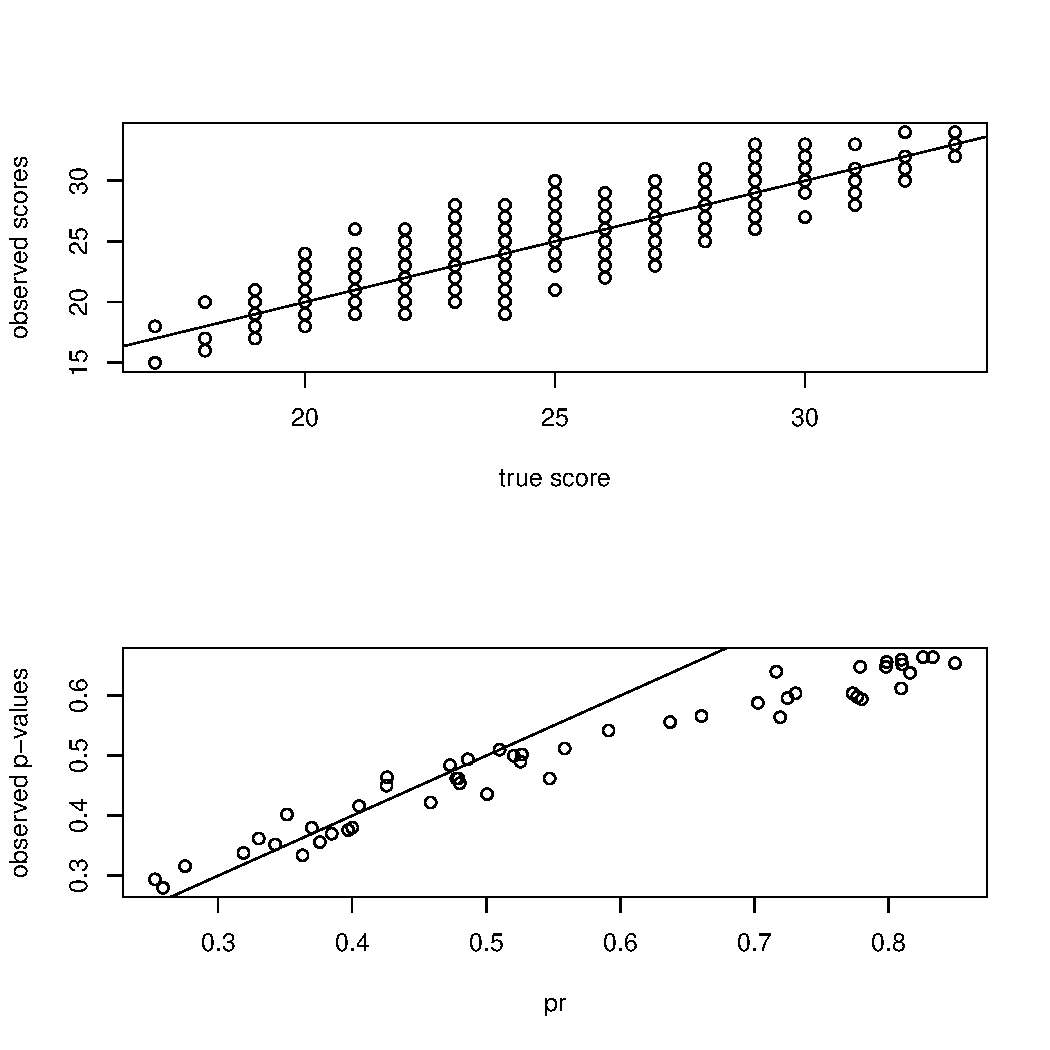
\includegraphics[width=\maxwidth]{figure/unnamed-chunk-2-1} 

\end{knitrout}

    These $\alpha$ plots make sense - they are centered around zero, as predicted, and as the number of items increases, $\alpha$ is more tightly clustered around zero.

  \subsection{Simulating Item Response Data}

\begin{knitrout}
\definecolor{shadecolor}{rgb}{0.969, 0.969, 0.969}\color{fgcolor}
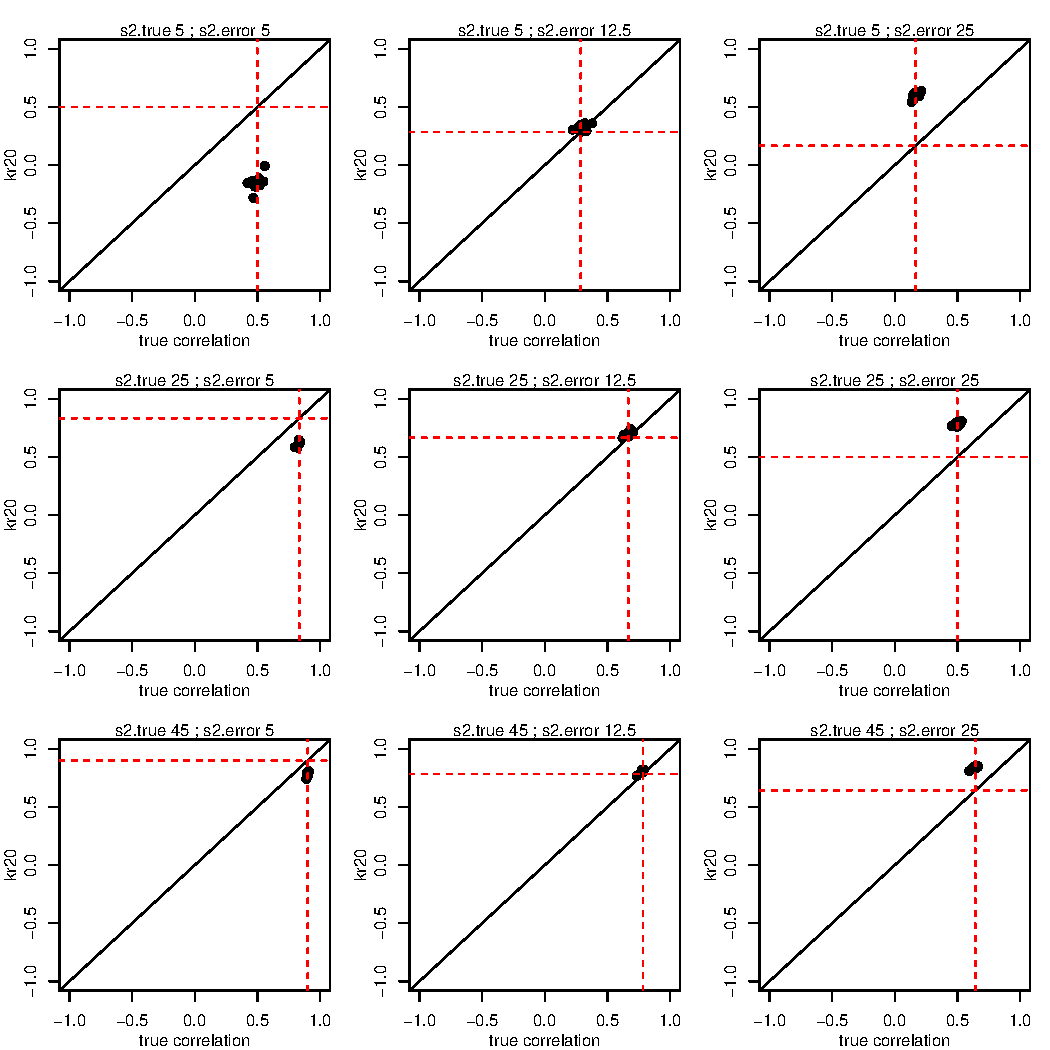
\includegraphics[width=\maxwidth]{figure/unnamed-chunk-3-1} 

\end{knitrout}

The feature of the data generation mechanism that makes the $\alpha$ values super low is that items are getting marked correctly (essentially) at random!  Even though the item responses generated correct p-values and test-level correlations, the data generation disregarded any internal structure you would expect.  More clearly stated, respondents of similar ability levels did not have similar item response profiles.

\begin{knitrout}
\definecolor{shadecolor}{rgb}{0.969, 0.969, 0.969}\color{fgcolor}
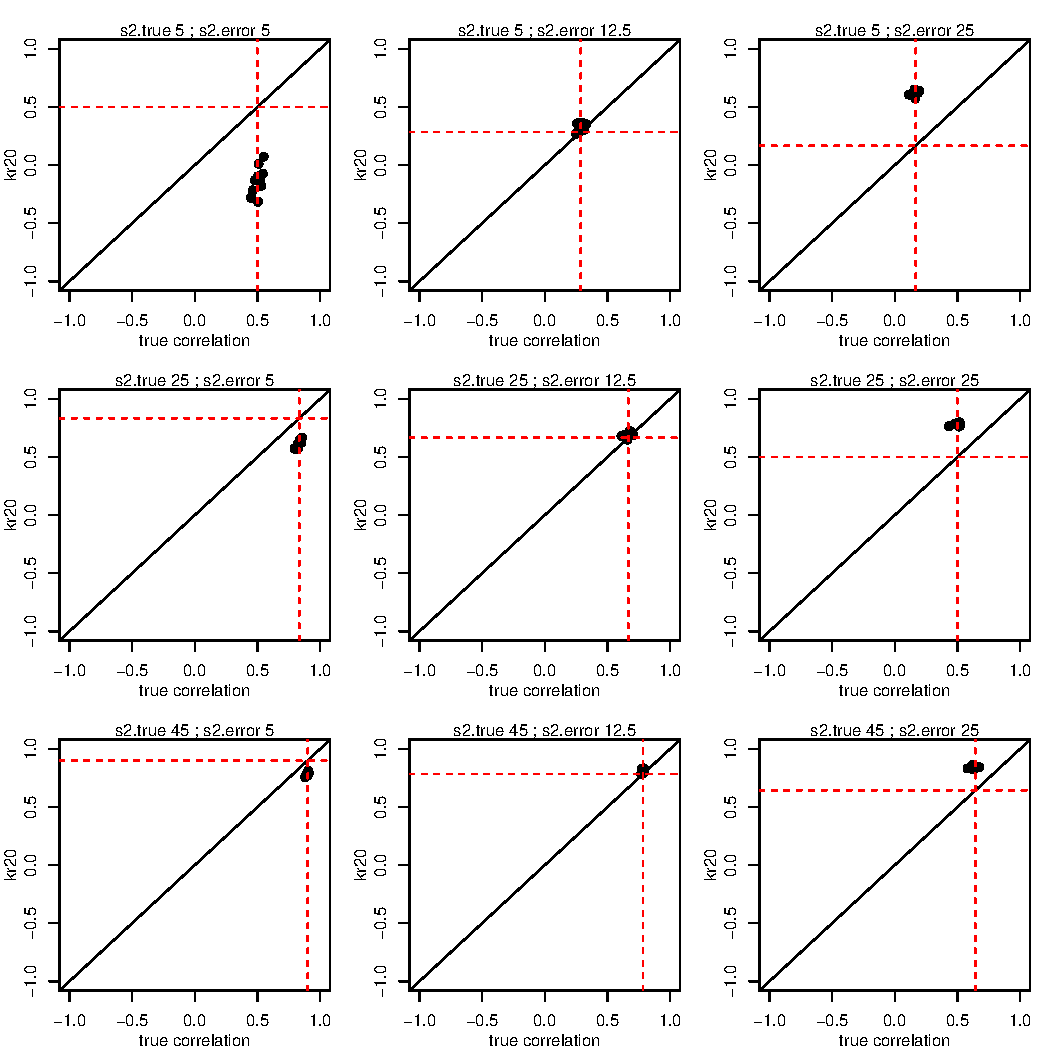
\includegraphics[width=\maxwidth]{figure/unnamed-chunk-4-1} 

\end{knitrout}

Looking at the resulting plots, it's clear that even with nonsensical item response data, the KR-20 estimate of reliability increases as a function of both true score variance and error variance.  This \em feels \em very wrong.  Increasing true score variance can be done by applying an instrument to a population it may not have been originally designed for.  Increasing error variance can be done by adding more items or manipulating the quality of items.  The challenge with feeling good about the CTT model is that KR-20 is both heavily valued and easily manipulated.  The worst part is that some of the behaviors that would increase a KR-20 value could have negative impacts on the validity of the instrument.

\pagebreak
\section{Basic Structure of IR Models}
\begin{enumerate}
\item
\begin{knitrout}
\definecolor{shadecolor}{rgb}{0.969, 0.969, 0.969}\color{fgcolor}
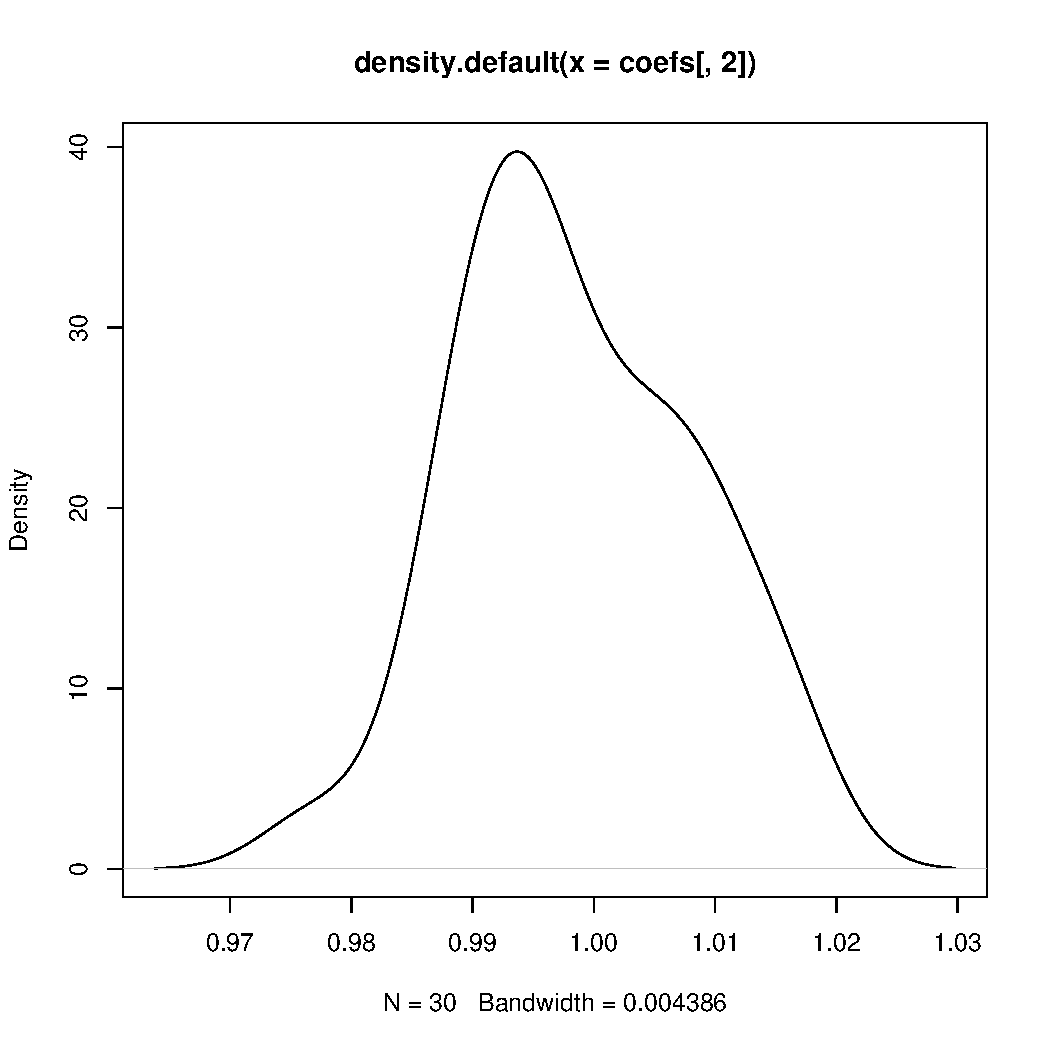
\includegraphics[width=\maxwidth]{figure/unnamed-chunk-5-1} 

\end{knitrout}
The plot shows the density of the item discriminations (i.e. the coefficients of the thetas in the equation $\beta_0 + \beta_1 \theta$), which means the density of the items' discrinations. The more the sample size is increased, the closer it appears to a normal distribution with a mean at 1. That means the discriminations are near 1. This makes sense because earlier in the code, we had set
\begin{knitrout}
\definecolor{shadecolor}{rgb}{0.969, 0.969, 0.969}\color{fgcolor}\begin{kframe}
\begin{alltt}
\hlstd{a} \hlkwb{<-} \hlnum{1}
\end{alltt}
\end{kframe}
\end{knitrout}
and a is the item discrimination coefficient.


\item
\begin{knitrout}
\definecolor{shadecolor}{rgb}{0.969, 0.969, 0.969}\color{fgcolor}
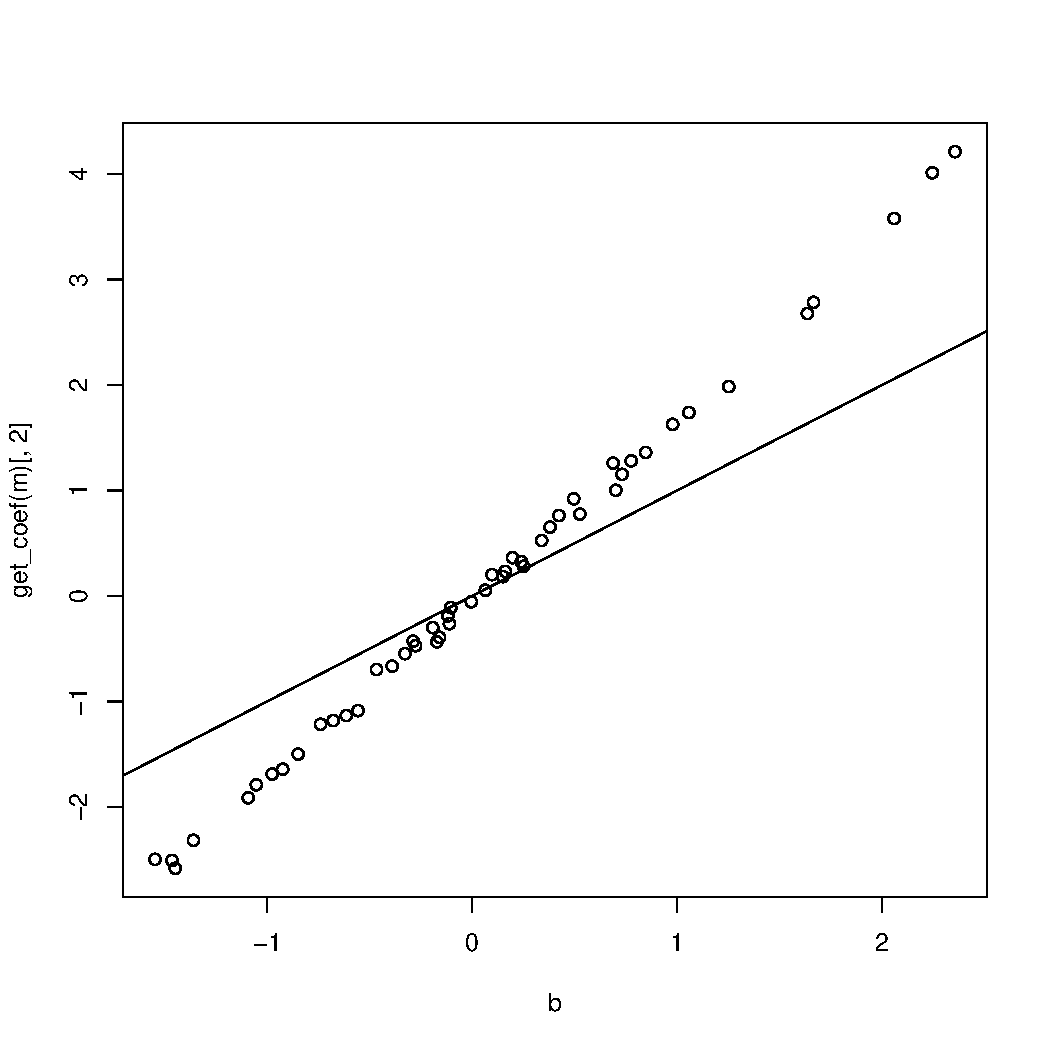
\includegraphics[width=\maxwidth]{figure/unnamed-chunk-7-1} 

\end{knitrout}
This plot shows that the b's are almost the same as the intercepts, which makes sense because it means that the actual item easiness is close to the estimated easiness.

\item
\begin{knitrout}
\definecolor{shadecolor}{rgb}{0.969, 0.969, 0.969}\color{fgcolor}
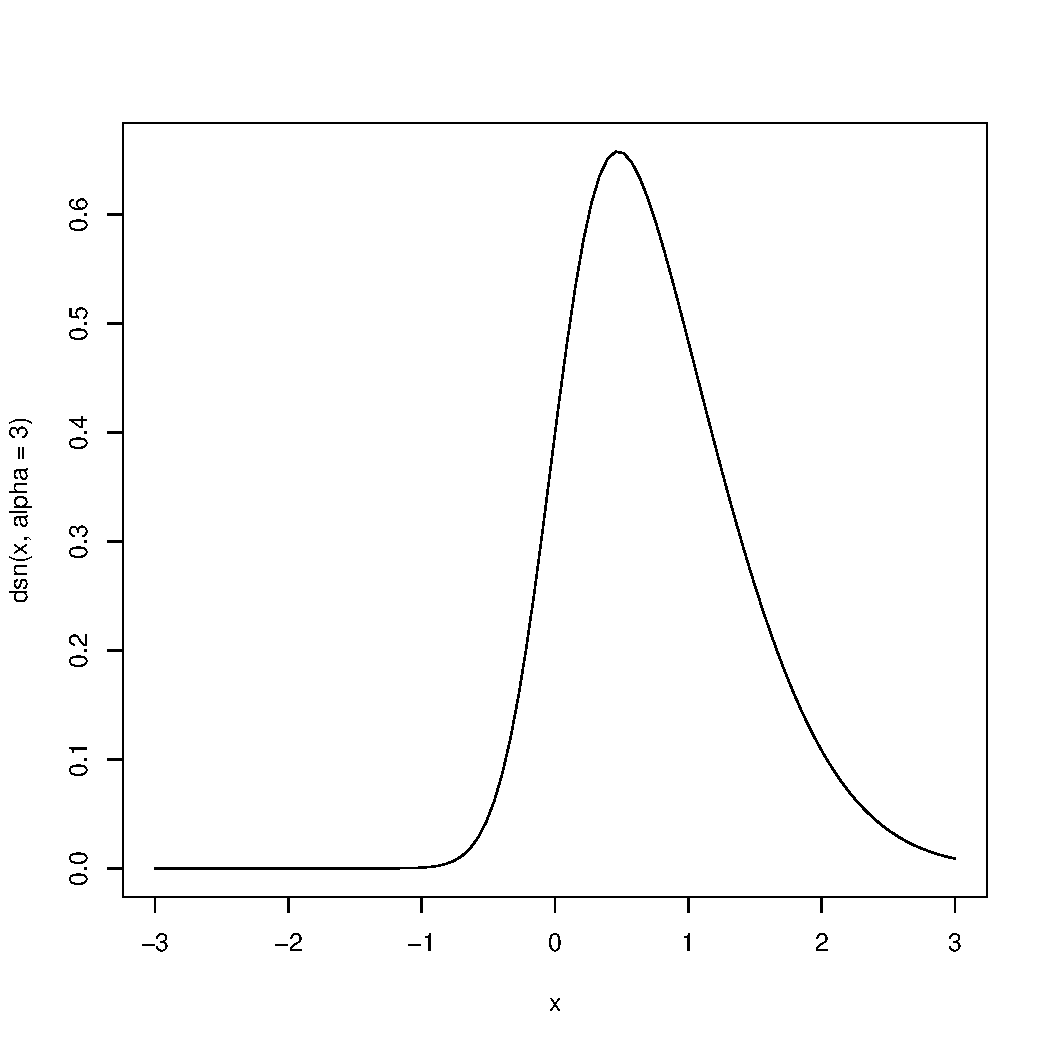
\includegraphics[width=\maxwidth]{figure/unnamed-chunk-8-1} 

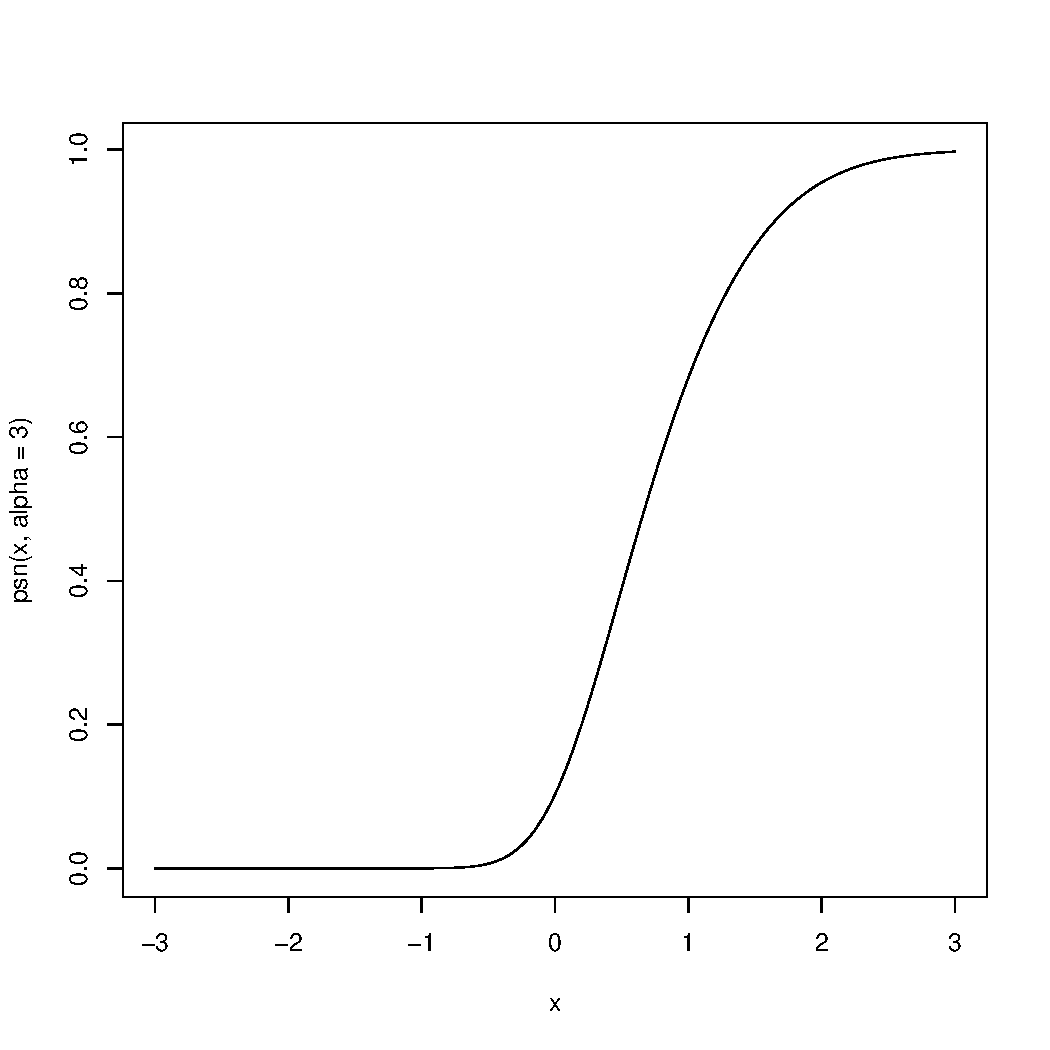
\includegraphics[width=\maxwidth]{figure/unnamed-chunk-8-2} 

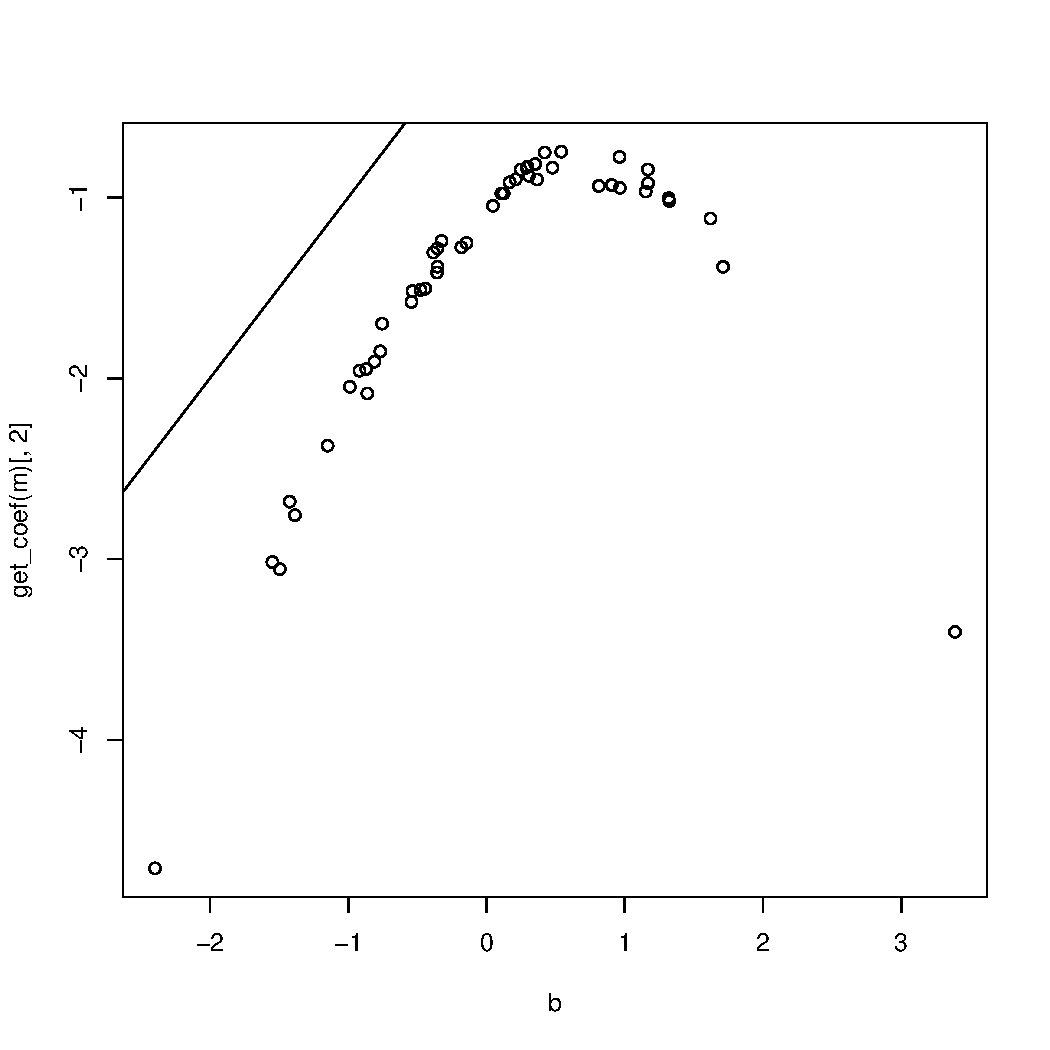
\includegraphics[width=\maxwidth]{figure/unnamed-chunk-8-3} 

\end{knitrout}
This is showing that when items get easier, the estimation gets worse and actually predicts that they're harder. 

\end{enumerate}

\section{Different Link Functions}
\subsection{The Default}
\begin{knitrout}
\definecolor{shadecolor}{rgb}{0.969, 0.969, 0.969}\color{fgcolor}
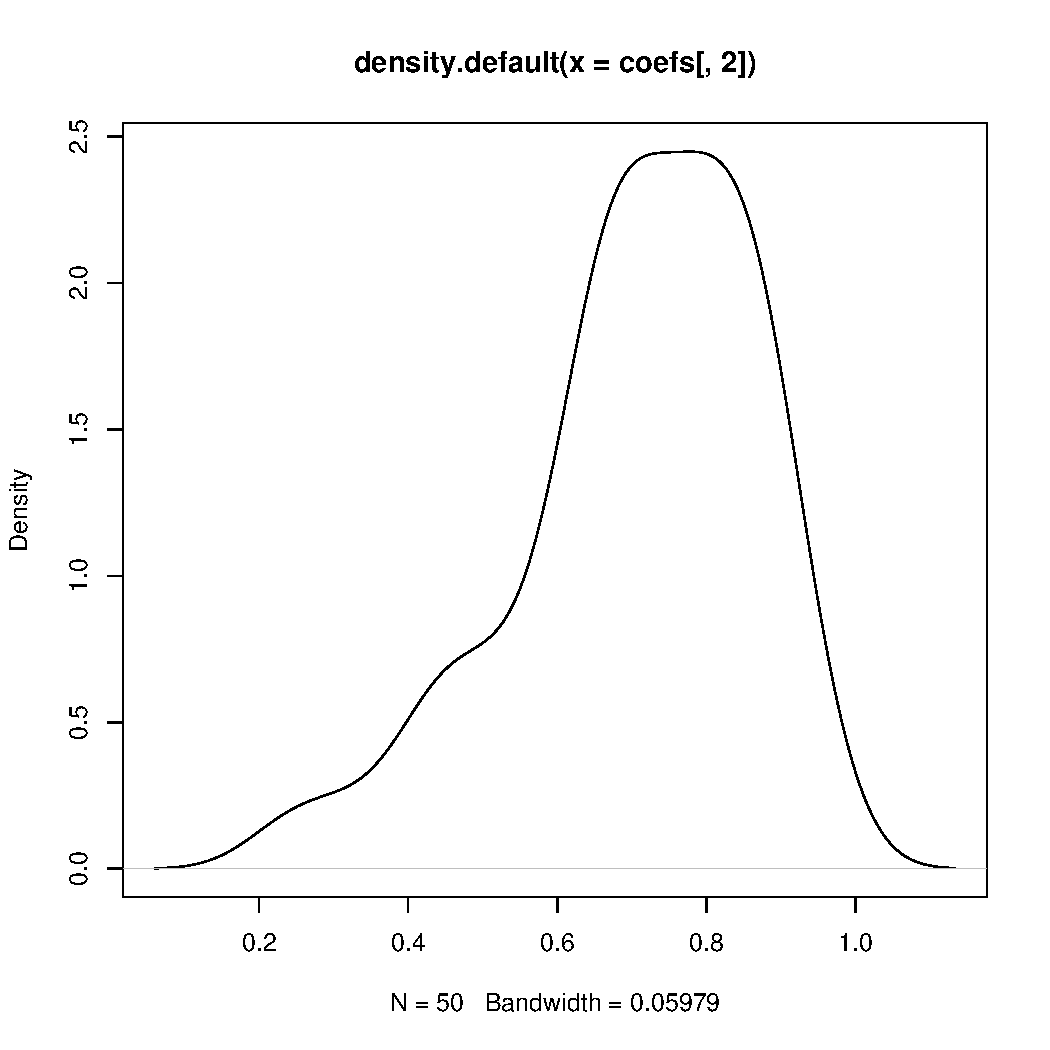
\includegraphics[width=\maxwidth]{figure/unnamed-chunk-9-1} 

\end{knitrout}

The default estimates item difficulties (or item easiness, specifically, because mirt) that are in line with the actual (specified) item difficulties.

\subsection{The Normal}

\begin{knitrout}
\definecolor{shadecolor}{rgb}{0.969, 0.969, 0.969}\color{fgcolor}
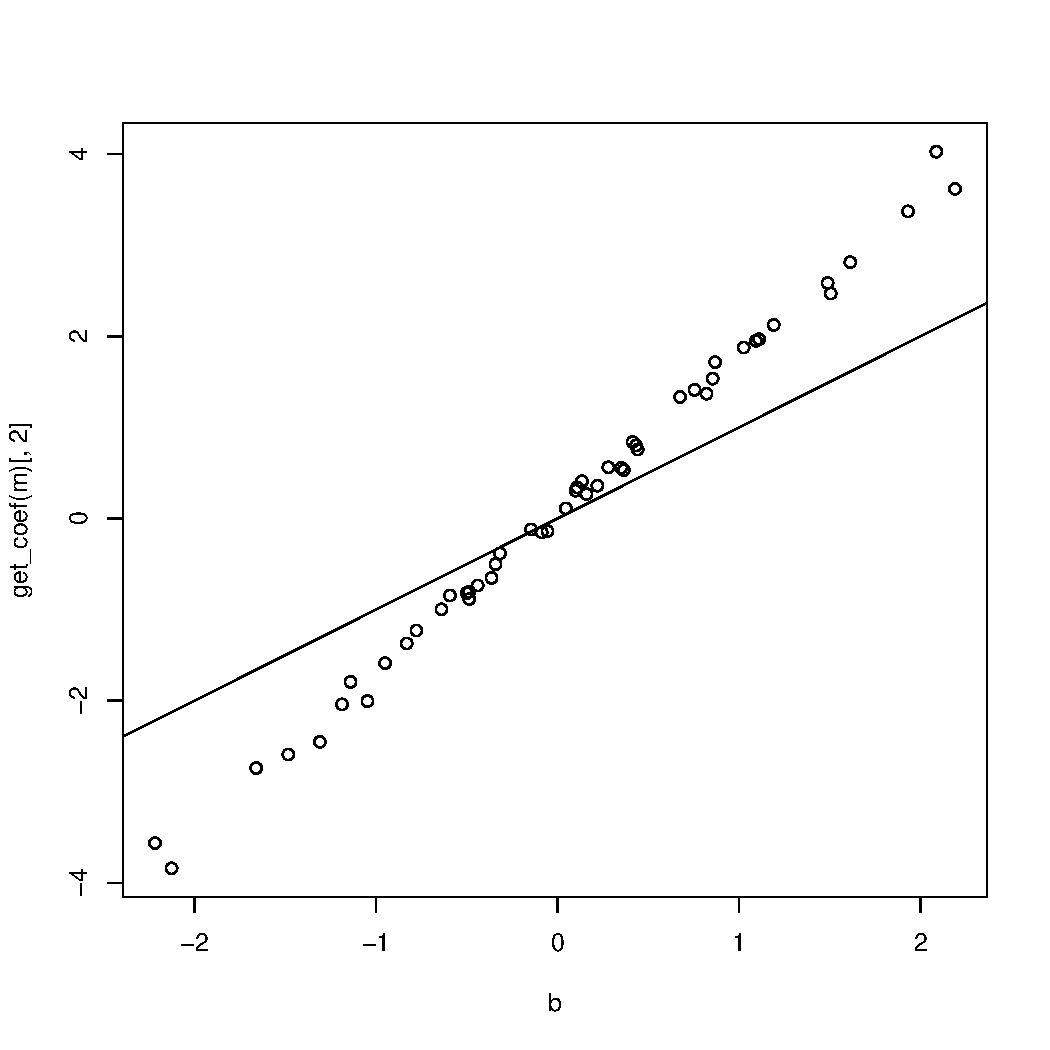
\includegraphics[width=\maxwidth]{figure/unnamed-chunk-10-1} 

\end{knitrout}

Using a normal link function, mirt predicts easy items are easier than they actually are and hard items are harder than they actually are.  The farther an item is from zero, the larger the gap between estimated difficulty and specified difficulty.  The slope of the line here is 1.7, so it is possible to transform between them, but the community tends to prefer the logistic because it is computationally simpler (even if the normal is theoretically nicer).

\subsection{Heavy Tails}

\begin{knitrout}
\definecolor{shadecolor}{rgb}{0.969, 0.969, 0.969}\color{fgcolor}
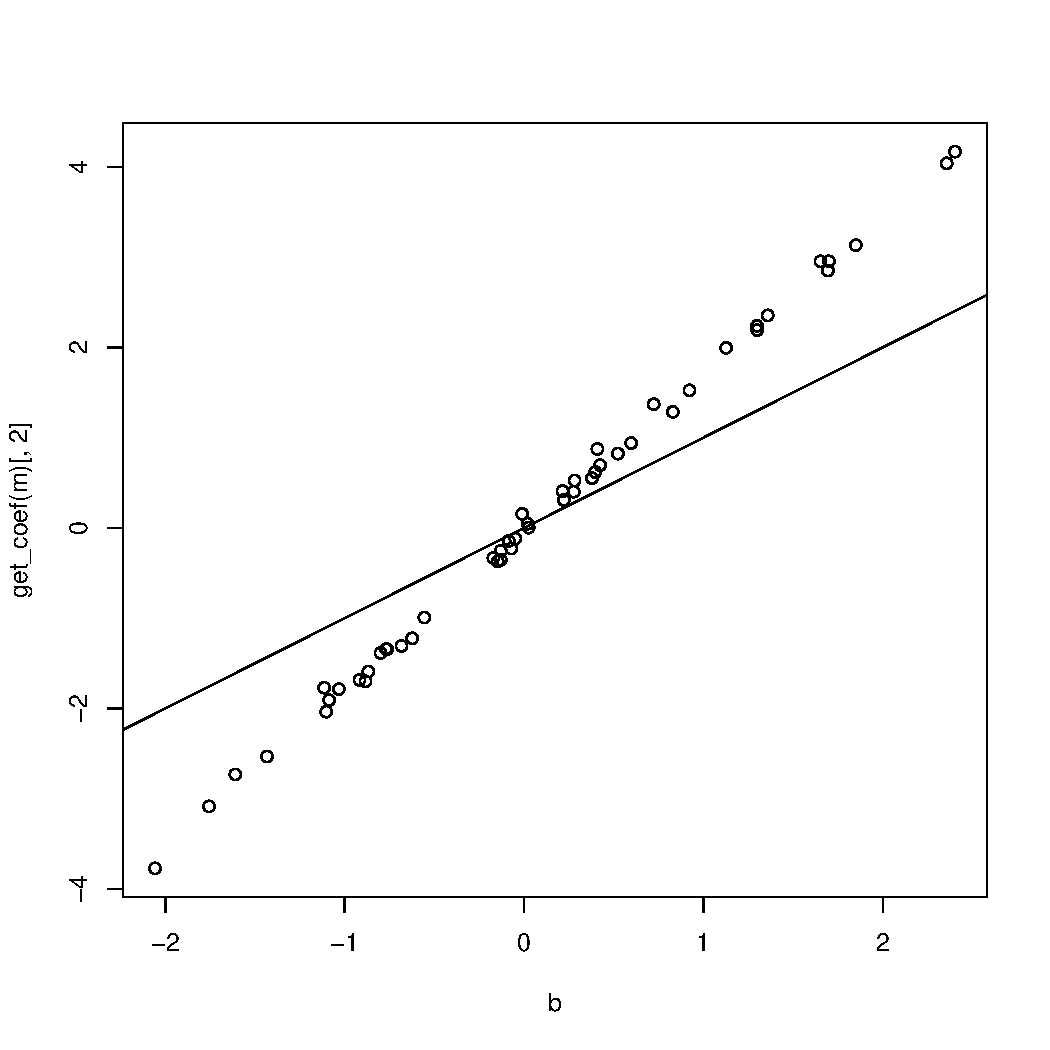
\includegraphics[width=\maxwidth]{figure/unnamed-chunk-11-1} 

\end{knitrout}

Using a link function with heavy tails, mirt does essentially the same as above, just with more divergence farther from zero.

\subsection{Skewed}

\begin{knitrout}
\definecolor{shadecolor}{rgb}{0.969, 0.969, 0.969}\color{fgcolor}
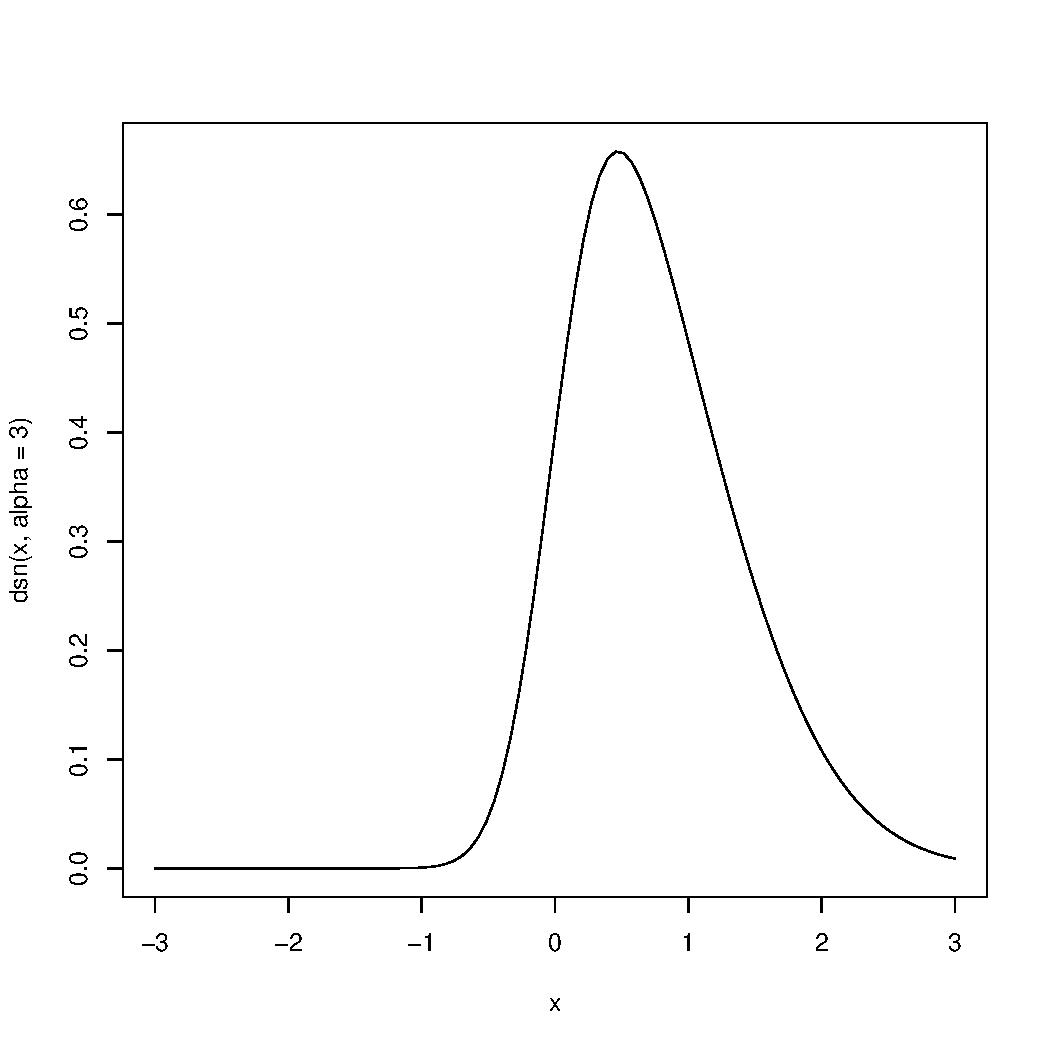
\includegraphics[width=\maxwidth]{figure/unnamed-chunk-12-1} 

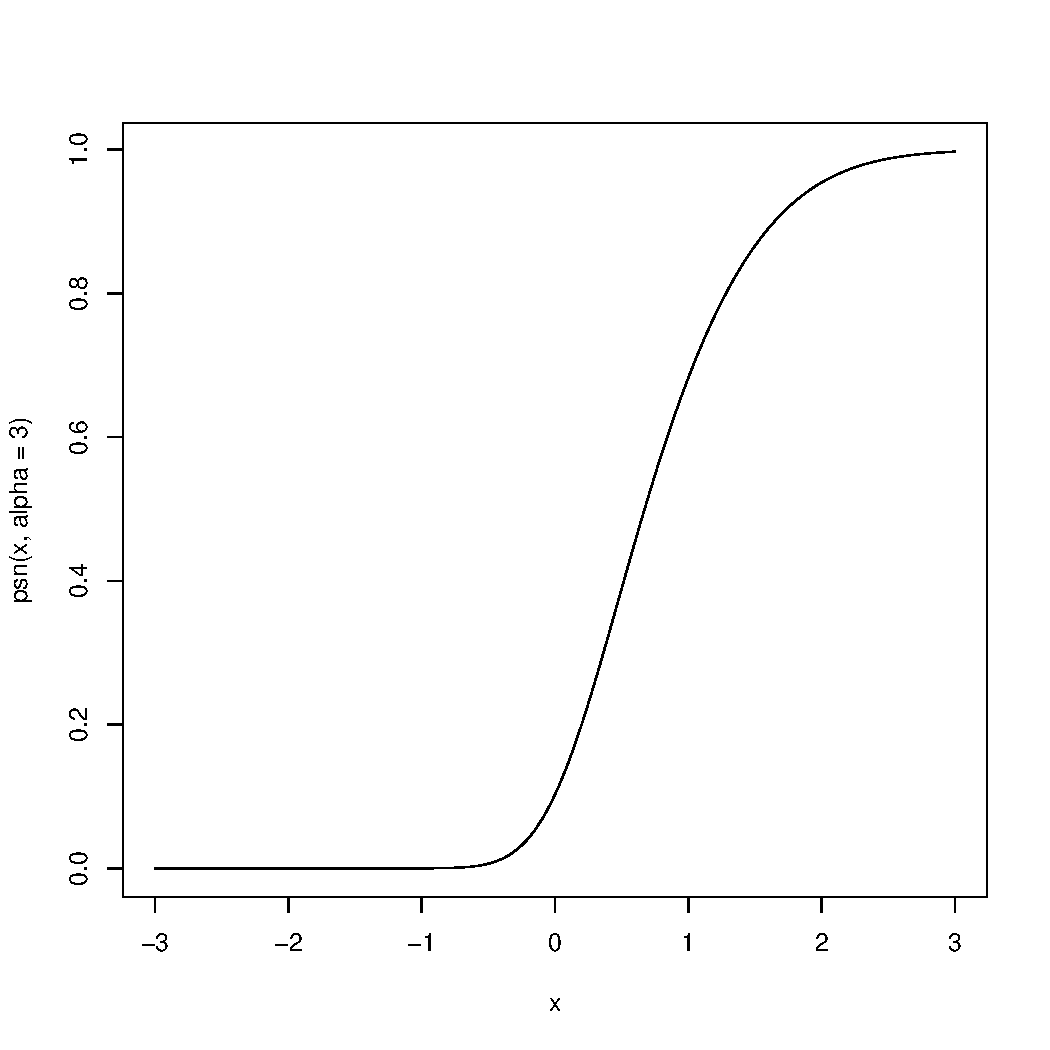
\includegraphics[width=\maxwidth]{figure/unnamed-chunk-12-2} 

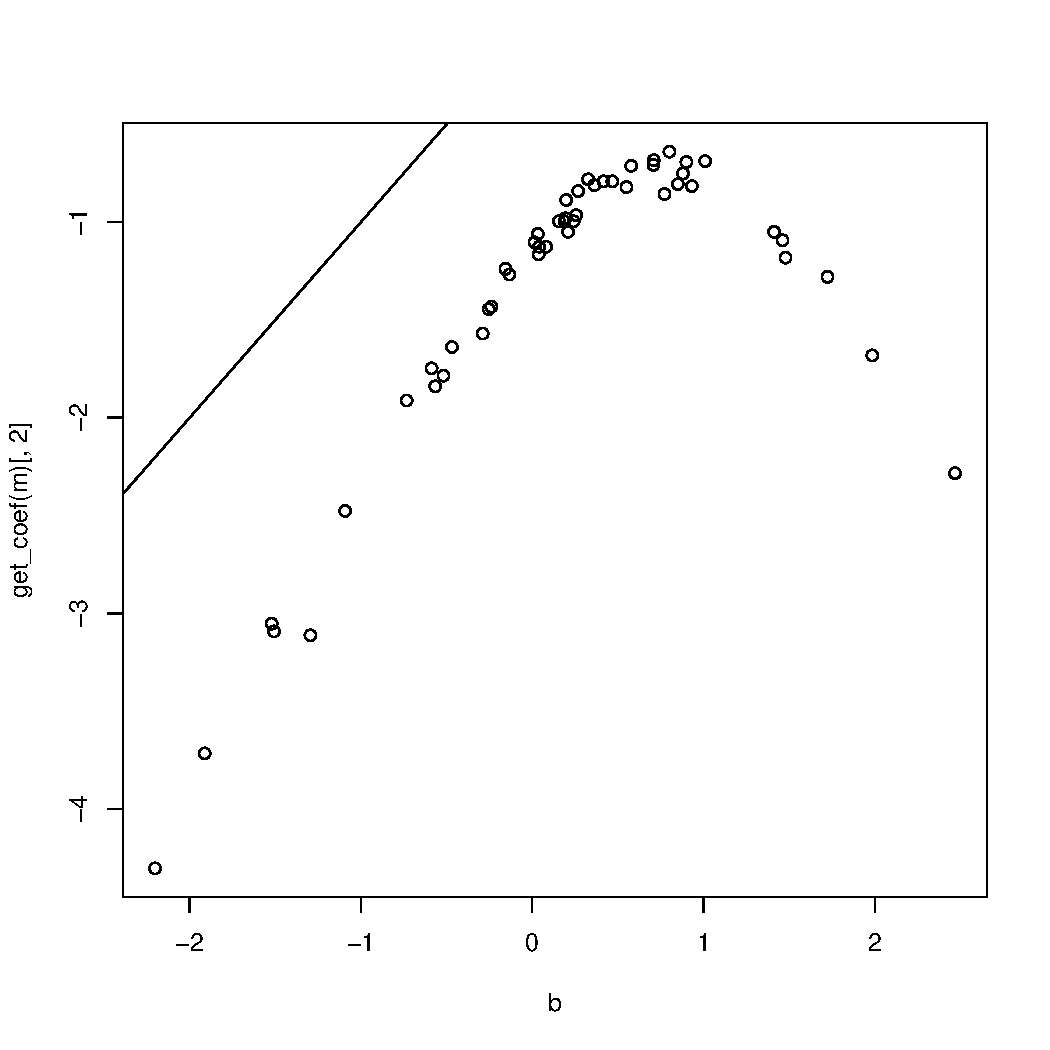
\includegraphics[width=\maxwidth]{figure/unnamed-chunk-12-3} 

\end{knitrout}

When using a skewed distribution as the link function, every item is estimated as being harder than it actually is, but where this model really tanks is for extremely easy items.  It finds those to be significantly harder than they actually are and the difference between actual and estimated difficulty for easy items diverges wildly.  The skew on the link function is set up in a way that there is essentially no impact of increased $\theta$ on the respondent's probability of getting the item correct until $\theta$ gets to a value of $-1$.  Remember that the input to the model is of the form $\theta_i + b_j$.  If trait values less than $-1$ don't provide any increase in probability of scoring correctly on an item, for items with easiness above $1$, the model will view those as significantly harder than they actually are.  If you look at the $b_estimated$ vs. $b$ curve, you can see that at $b =1$, the estimated easiness starts to take a turn away from actual easiness.  This is a product of the link function being non-symmetric, essentially causing the two halves of the graph to be scaled differently.

\pagebreak
\section{Adding A Lower Asymptote}

\begin{knitrout}
\definecolor{shadecolor}{rgb}{0.969, 0.969, 0.969}\color{fgcolor}
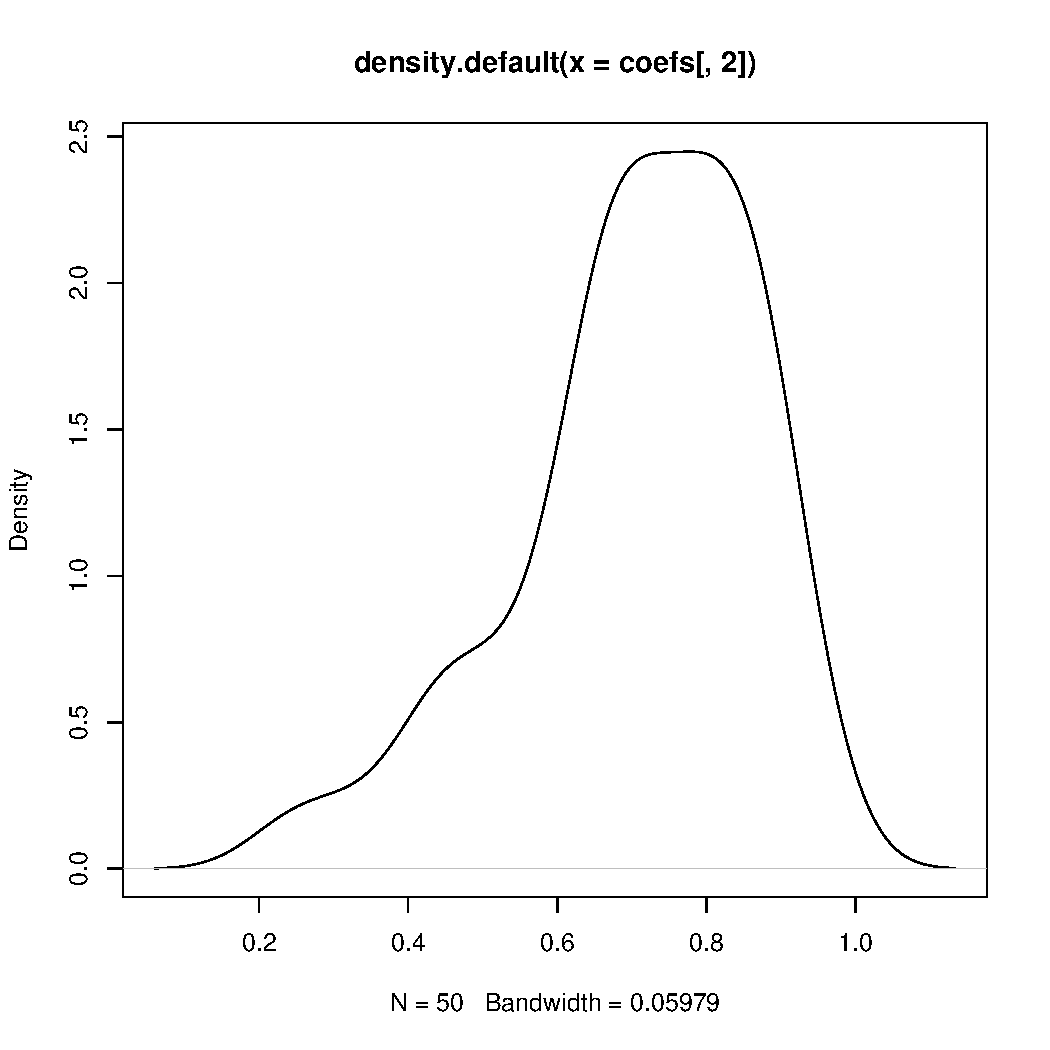
\includegraphics[width=\maxwidth]{figure/unnamed-chunk-13-1} 

\end{knitrout}

When moving the lower asymptote above zero, we simulate guessing.  In the original model, with no guessing parameter, the discrimination density plot was centered around 1.  Now, it is centered around 0.75.  This happens because raising the floor of the logistic curve fundamentally changes its shape, lowering the discrimination.

\begin{knitrout}
\definecolor{shadecolor}{rgb}{0.969, 0.969, 0.969}\color{fgcolor}
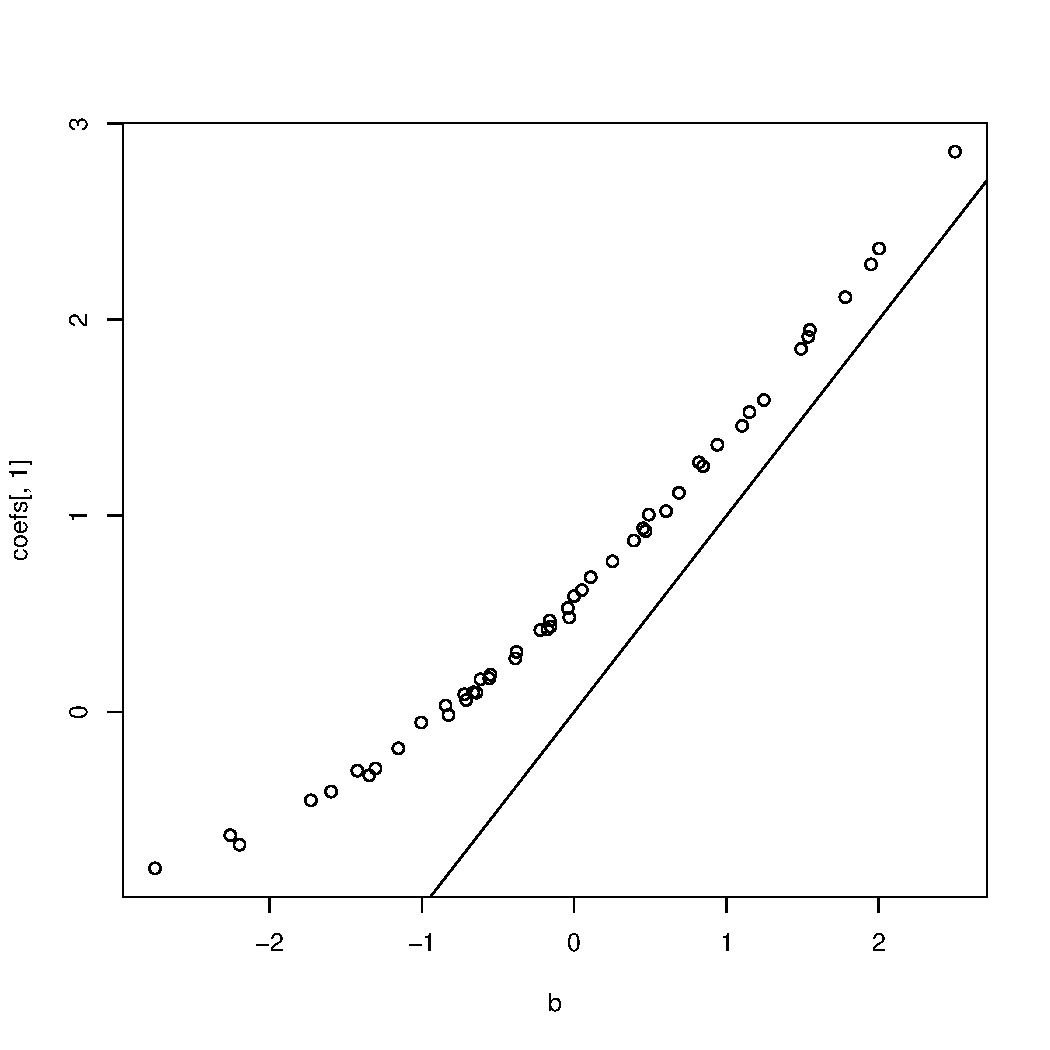
\includegraphics[width=\maxwidth]{figure/unnamed-chunk-14-1} 

\end{knitrout}

When looking at the item easiness estimates, the model overestimates easiness.  This is especially true for the harder questions(easiness less than zero), where the estimate starts to diverge from the actual difficulty.  One explanation for this is that for harder questions, a larger segment of the population is benefiting from guessing, where on easier questions, a smaller segment of the population benefits from guessing (because they were already getting that item correct).

\end{document}
